\chapter{Proposed solution}
\label{chapter:proposedSolution}

\section{Approach definition}
\label{section:approachDefinition}

Now that we have analyzed the technical requirements and identified some of the challenges that could be encountered, we can continue with defining the solution for the described problem. Our approach would involve designing and developing a web application, keeping in mind its advantages over desktop applications, which we described in the previous section. The app would include two major parts: a web service developed in Java using the Spring Boot Framework and a client app built using the ReactJS Framework. The web sevice will define a REST API which will be used for communication between the client and the server. It will also handle the business logic and manage the persistence of data, which will be achieved by using a MySQL database. The client app will be the one that will run in the user's browser. As REST is stateless by definition, the client app will have to manage the session state. This will be achieved with the help of Redux - a predictable state containerfor JavaScript apps.

One important thing to keep in mind is that the application will be used for managing real documents of a public institution, which could potentially involve sensitive data. To secure our app, we will use features offered by Spring Security to enable JSON Web Token Authentication and manage access control.


\section{Technologies used}
\label{section:technologiesUsed}

In the following subsections of this chapter we will describe each of the chosen technologies in detail, with a strong focus on features that were decisive in choosing it over alternative technologies from the same branch.


\subsection{The Spring Framework}
\label{subsection:theSpringFramework}

The Spring Framework is an application framework for the Java platform which offers a wide range of features for modern Java-based enterprise applications. According to a survey from 2018, Spring is the most popular Web Framework worldwide in the JVM ecosystem (See Figure \ref{javaWebFrameworksTrendsImg}). It provides a large set of functionality and tools, making it suitable for a big variety of applications. In addition,  its flexibility and focus on ease of use allow developers to focus on the application business logic rather than configurations and boilerplate code, thus increasing velocity, productivity and development speed.

\begin{figure}[H]
    \centering
    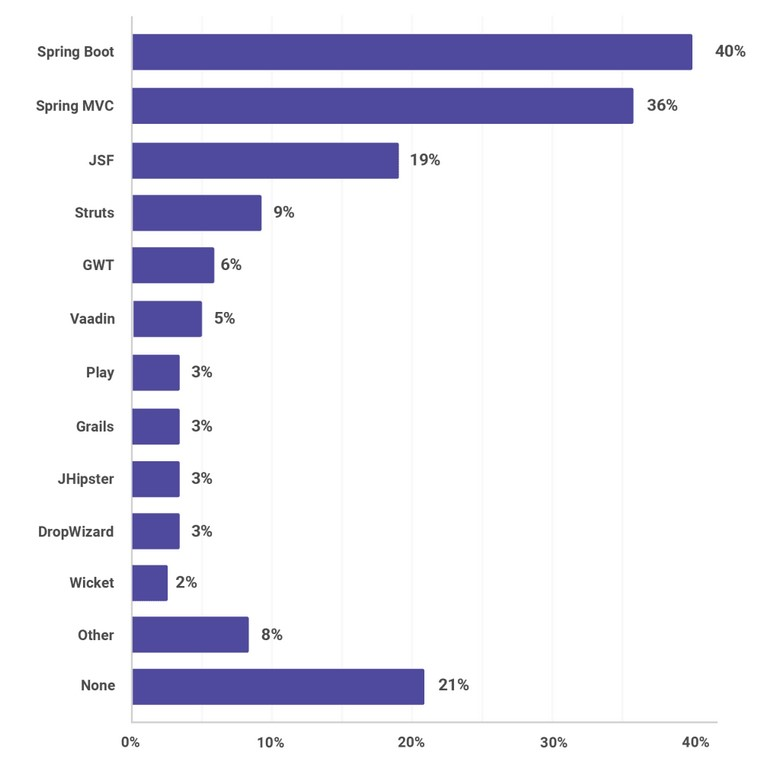
\includegraphics[width=4in]{images/javaWebFrameworksTrends}
    \caption{The most popular Java Web Frameworks according to the JVM Ecosystem report 2018 \cite{jvmEcosystemReport}}
    \label{javaWebFrameworksTrendsImg}
\end{figure}

One of the most important features offered by Spring is \textit{Inversion of Control} (IoC), achieved by \textit{Dependency Injection} (DI). According to this principle, objects are not responsible for creating their dependencies. Instead, they should be "injected" into the object through arguments passed to the constructor, setter methods or factory methods. In contrast to the classical way where each object is locating and instantiating all of its dependencies, the DI approach has several advantages. The most important one is achiving loose coupling, making it easier to interchange distinct implementations and maintain program modularity.

To achieve this, the Spring Framework uses an \textit{IoC container}. It is responsible for the instantiation, configuration and managing of the \textit{beans} - objects that will be used by the application (See Figure \ref{springIocContainer}). In order to know how each bean should be created and which dependencies injected, the IoC container needs additional configuration information. This is provided as metadata in form of XML, Java Configuration classes or Java annotations. In our project, we are going to use Java annotations as it is the most easy and straightforward way to configure beans.

\begin{figure}[H]
    \centering
    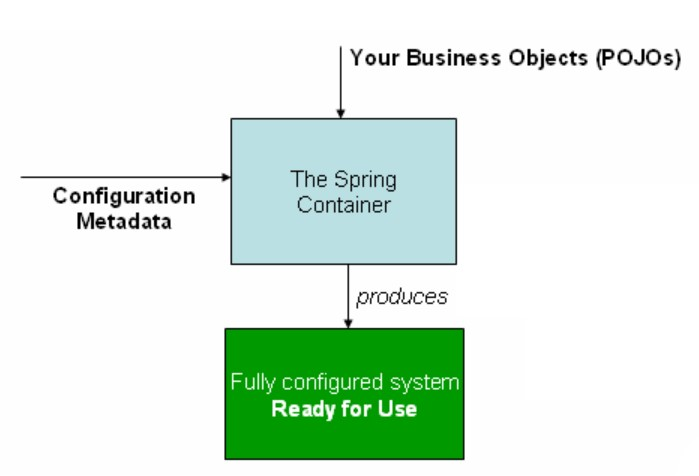
\includegraphics[width=4in]{images/springIocContainer}
    \caption{The Spring IoC Container \cite{springDocs}}
    \label{springIocContainer}
\end{figure}


% The org.springframework.context.ApplicationContext interface represents the Spring IoC container and is responsible for instantiating, configuring, and assembling the beans. The container gets its instructions on what objects to instantiate, configure, and assemble by reading configuration metadata. The configuration metadata is represented in XML, Java annotations, or Java code. It lets you express the objects that compose your application and the rich interdependencies between those objects.

% As the preceding diagram shows, the Spring IoC container consumes a form of configuration metadata. This configuration metadata represents how you, as an application developer, tell the Spring container to instantiate, configure, and assemble the objects in your application.



% In Spring, the objects that form the backbone of your application and that are managed by the Spring IoC container are called beans. A bean is an object that is instantiated, assembled, and otherwise managed by a Spring IoC container. Otherwise, a bean is simply one of many objects in your application. Beans, and the dependencies among them, are reflected in the configuration metadata used by a container.


% Spring’s flexible and comprehensive set of extensions and third-party libraries let developers build almost any application imaginable. At its core, Spring Framework’s Inversion of Control (IoC) and Dependency Injection (DI) features provide the foundation for a wide-ranging set of features and functionality. Whether you’re building secure, reactive, cloud-based microservices for the web, or complex streaming data flows for the enterprise, Spring has the tools to help.

% A key element of Spring is infrastructural support at the application level: Spring focuses on the "plumbing" of enterprise applications so that teams can focus on application-level business logic, without unnecessary ties to specific deployment environments.


% //
% Spring makes building web applications fast and hassle-free. By removing much of the boilerplate code and configuration associated with web development, you get a modern web programming model that streamlines the development of server-side HTML applications, REST APIs, and bidirectional, event-based systems.





% Singleton pattern
% Factory Method pattern
% Proxy pattern
% Template pattern



% https://blog.eduonix.com/java-programming-2/learn-design-patterns-used-spring-framework/

\subsection{Spring Boot}
\label{subsection:springBoot}

\subsection{Spring Security}
\label{subsection:proposedSolution}

\subsection{Spring JDBC}
\label{subsection:springJDBC}

\subsection{ReactJS Framework}
\label{section:reactJSFramework}

\subsection{Redux}
\label{section:redux}

\subsection{MySQL Database}
\label{section:mysqlDatabase}

% - performance (big amount of data)
% - relational vs non-relational db
% - where to store files? (db vs cloud)
% - db stuff (indexing / speeding up things ? highPerformanceMySQL)
% There's usually a lot of data, a moderate system will have over 1GB of data
% organized in tens of millions of records, so much data that managing it is a major part
% of the system. Older systems used indexed file structure such as IBM's VSAM and
% ISAM. Modern systems usually use databases, mostly relational databases. The
% design and feeding of these databases has turned into a sub-profession of its own.




% just so items from .bib would show up in bibliography
\cite{buildingRESTfulWebServicesWithSpring}
\cite{tamingTheStateInReact}
\cite{highPerformanceMySQL}


